\documentclass[a4paper,12pt]{article}

\usepackage[T1]{fontenc}
\usepackage[utf8]{inputenc}
\usepackage[english, polish]{babel}
\usepackage{lmodern}
\usepackage{graphicx}
\usepackage{fancyhdr}
\usepackage{float}
\usepackage{array}
\usepackage{hyperref}
%\usepackage{mathtools}


\setlength{\textheight}{23.5cm}
\setlength{\textwidth}{15.92cm}
\setlength{\footskip}{10mm		}
\setlength{\oddsidemargin}{0mm}
\setlength{\evensidemargin}{0mm}
\setlength{\topmargin}{0mm}
\setlength{\headsep}{15mm}
\setlength{\parindent}{0cm}
\setlength{\parskip}{2.5mm}
%nowa extra row do tabeli :)  :) 
\setlength{\extrarowheight}{4pt}

\author{Justyna Ilczuk, Patryk Lipka-Bartosik}

\begin{document}

\begin{center}

    \begin{tabular}{ | m{5cm}| m{5cm} | m{5cm} |}
    \hline 
    \multicolumn{2}{|c|}{{ \Large \textbf{Laboratorium Fizyki 3}} }
    &  
    \begin{center}
    Data wykonania ćwiczenia:
    \end{center}
    \begin{center}
      marzec-kwiecień 2014 
    \end{center}
    \begin{center}
    Wtorek 9.45-17.45
    \end{center}
     \\ 
    
    \hline
    \multicolumn{2}{|c|}{Justyna Ilczuk \newline Patryk Lipka-Bartosik}
    & \begin{center}
    {\small Data złożenia sprawozdania:} \newline \today
    \end{center}   \\
   	
   	\hline
    Wydział Fizyki & Specjalność: Fizyka Komputerowa \newline Rok akademicki: 2013/2014 &    Laboratorium naukowe \\
   	\hline
   	\multicolumn{2}{|l|}{Prowadzący: Irena Gronowska} & \multicolumn{1}{|l|}{Ocena końcowa:}\\
    \hline
    \end{tabular}
\end{center}

\newpage

\pagestyle{fancy}
\fancyfoot[CO]{\ }
\fancyhead[RO]{\footnotesize{\thepage} }
%\fancyhead[RO]{\footnotesize{\ } }

% wrzucanie wykresów:

%\begin{figure} [H]
%  \begin{center}
%    \includegraphics[width = 15cm]{Rysunek.png}
%    \caption{Układ pomiarowy}
%  \end{center}
%\end{figure}

\section{Cel ćwiczenia}

Celem ćwiczenia było jak zmienia się struktura mięsa pod wpływem wysokiego ciśnienia i zmierzenie w mięsie prędkości rozchodzenia się fali przed i po zgniataniu. 

\section{Wstęp}

Badaliśmy mięso.


\section{Użyty sprzęt i układy pomiarowe}

Do przeprowadzenia eksperymentu używaliśmy: 

\begin{enumerate}
  \item Mikroskop akustyczny
  \item Komora wysokociśnieniowa
  
\end{enumerate}


\section{Opracowanie wyników}

%TODO add proper descriptions to this figures
Mieso1:


\begin{figure} [H]
  \begin{center}
    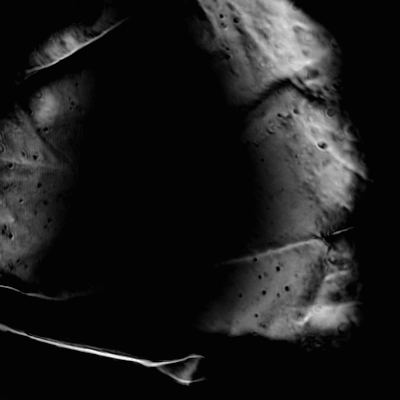
\includegraphics[width = 15cm]{data/MIESO1.png}
    \caption{Mięso}
  \end{center}
\end{figure}


\begin{figure} [H]
  \begin{center}
    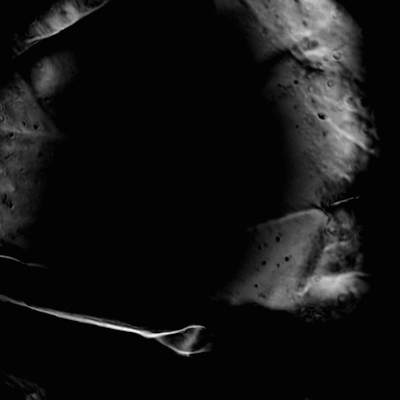
\includegraphics[width = 15cm]{data/MIESO2.png}
    \caption{Mięso}
  \end{center}
\end{figure}


\begin{figure} [H]
  \begin{center}
    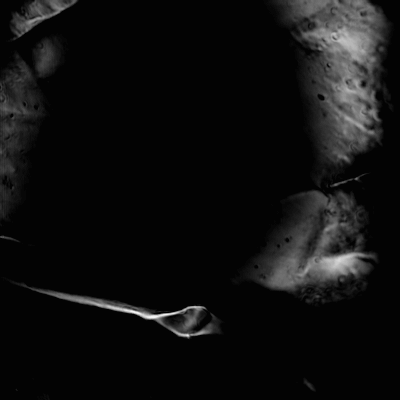
\includegraphics[width = 15cm]{data/MIESO3.png}
    \caption{Mięso}
  \end{center}
\end{figure}


Mieso2:

\begin{figure} [H]
  \begin{center}
    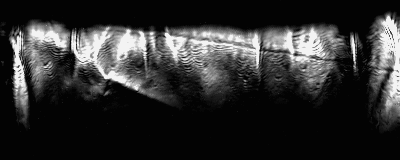
\includegraphics[width = 15cm]{data/2MIES0.png}
    \caption{Mięso}
  \end{center}
\end{figure}

\begin{figure} [H]
  \begin{center}
    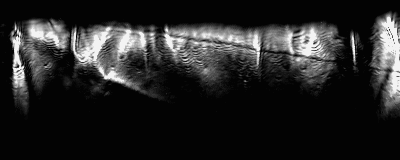
\includegraphics[width = 15cm]{data/2MIES1.png}
    \caption{Mięso}
  \end{center}
\end{figure}


\begin{figure} [H]
  \begin{center}
    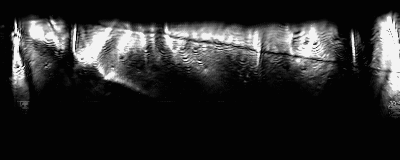
\includegraphics[width = 15cm]{data/2MIES2.png}
    \caption{Mięso}
  \end{center}
\end{figure}


\begin{figure} [H]
  \begin{center}
    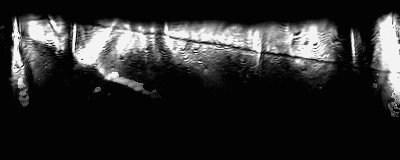
\includegraphics[width = 15cm]{data/2MIES3.png}
    \caption{Mięso}
  \end{center}
\end{figure}


Mieso3:

\begin{figure} [H]
  \begin{center}
    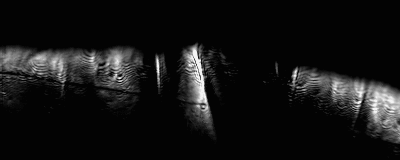
\includegraphics[width = 15cm]{data/4MIES1.png}
    \caption{Mięso}
  \end{center}
\end{figure}


\begin{figure} [H]
  \begin{center}
    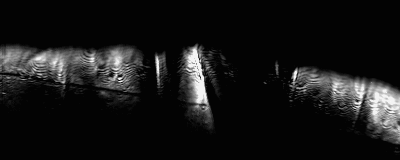
\includegraphics[width = 15cm]{data/4MIES2.png}
    \caption{Mięso}
  \end{center}
\end{figure}

Mieso 5:

\begin{figure} [H]
  \begin{center}
    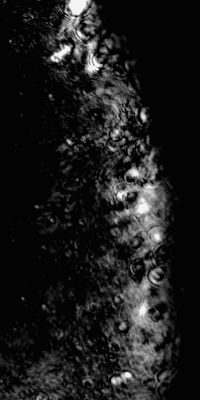
\includegraphics[width = 15cm]{data/5MIES1.png}
    \caption{Mięso}
  \end{center}
\end{figure}

\begin{figure} [H]
  \begin{center}
    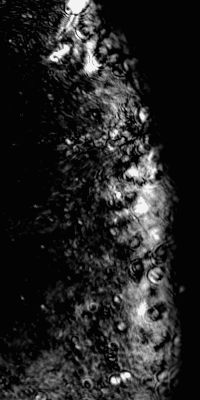
\includegraphics[width = 15cm]{data/5MIES2.png}
    \caption{Mięso}
  \end{center}
\end{figure}


\begin{figure} [H]
  \begin{center}
    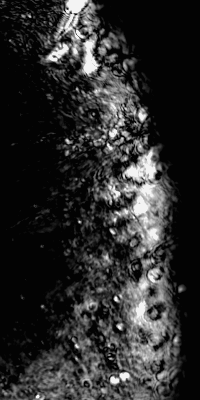
\includegraphics[width = 15cm]{data/5MIES3J.png}
    \caption{Mięso}
  \end{center}
\end{figure}


\begin{figure} [H]
  \begin{center}
    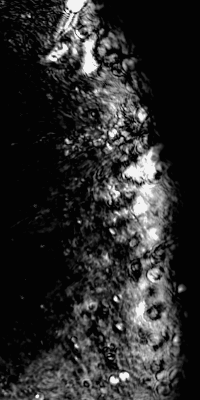
\includegraphics[width = 15cm]{data/5MIES4J.png}
    \caption{Mięso}
  \end{center}
\end{figure}



\section{Wnioski}


%{\Large Hipoteza potwierdzona, ta fizyka jest szalona! }

%\section {Źródła dodatkowe}
  
 %kosmos i obserwacja losowych zachować w koloniach mrówek. 

\end{document}